\begin{figure}[htp]
	\begin{center}
	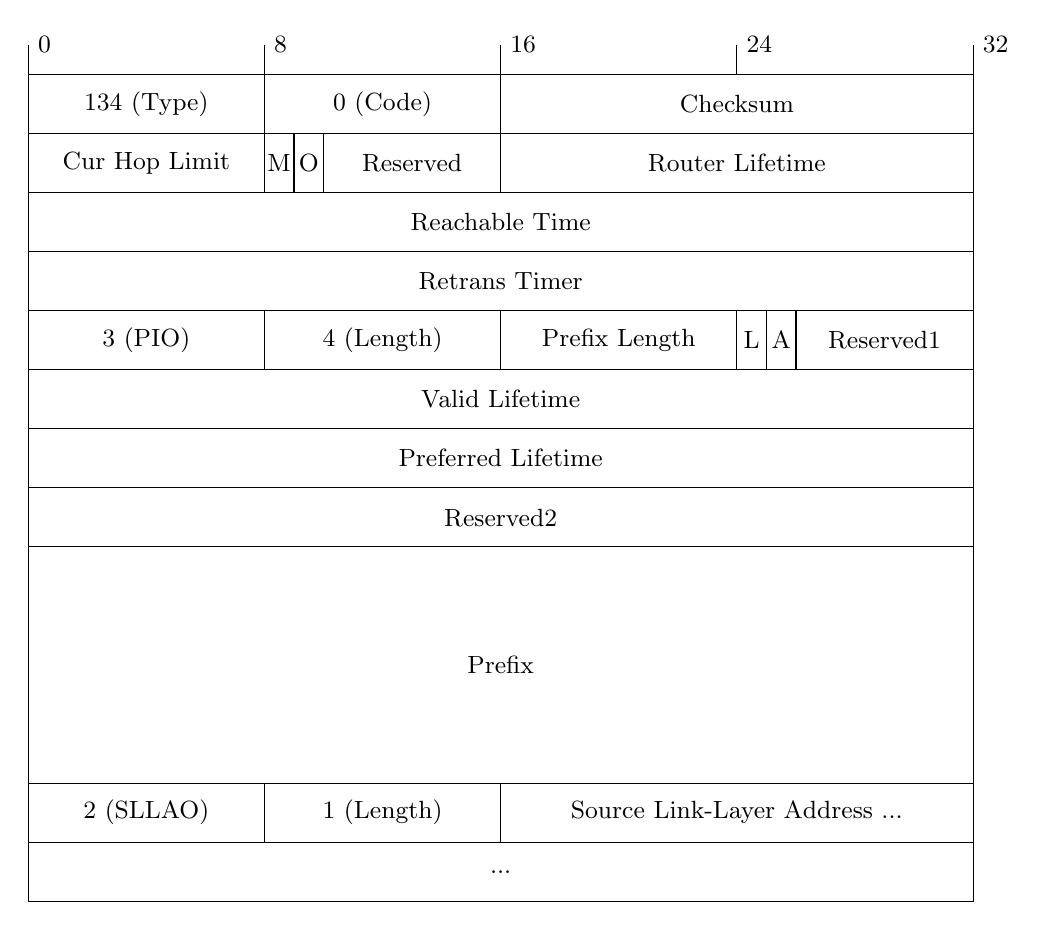
\begin{tikzpicture}[scale=0.75]
		\draw (0,0) rectangle (16,14);
		\draw (0,14) -- ++(0,0.5) node[right] {\small 0};
		\draw (4,14) -- ++(0,0.5) node[right] {\small 8};
		\draw (8,14) -- ++(0,0.5) node[right] {\small 16};
		\draw (12,14) -- ++(0,0.5) node[right] {\small 24};
		\draw (16,14) -- ++(0,0.5) node[right] {\small 32};
0
		\draw (4,13) -- ++(0,1);
		\node at (2,13.5) {\small 134 (Type)};
		\draw (8,13) -- ++(0,1);
		\node at (6, 13.5) {\small 0 (Code)};
		\node at (12, 13.5) {\small Checksum};
		\draw (0,13) -- ++(16,0);

		\draw (4,12) -- ++(0,1);
		\node at (2, 12.5) {\small Cur Hop Limit};
		\draw (4.5,12) -- ++(0,1);
		\node at (4.25, 12.5) {\small M};
		\draw (5,12) -- ++(0,1);
		\node at (4.75, 12.5) {\small O};
		\draw (8,12) -- ++(0,1);
		\node at (6.5, 12.5) {\small Reserved};
		\node at (12, 12.5) {\small Router Lifetime};
		\draw (0,12) -- ++(16,0);

		\node at (8, 11.5) {\small Reachable Time};
		\draw (0,11) -- ++(16,0);

		\node at (8, 10.5) {\small Retrans Timer};
		\draw (0,10) -- ++(16,0);

		\draw (4,9) -- ++(0,1);
		\node at (2,9.5) {\small 3 (PIO)};
		\draw (8,9) -- ++(0,1);
		\node at (6, 9.5) {\small 4 (Length)};
		\draw (12,9) -- ++(0,1);
		\node at (10, 9.5) {\small Prefix Length};
		\draw (12.5,9) -- ++(0,1);
		\node at (12.25, 9.5) {\small L};
		\draw (13,9) -- ++(0,1);
		\node at (12.75, 9.5) {\small A};
		\node at (14.5, 9.5) {\small Reserved1};
		\draw (0,9) -- ++(16,0);

		\node at (8,8.5) {\small Valid Lifetime};
		\draw (0,8) -- ++(16,0);
		\node at (8,7.5) {\small Preferred Lifetime};
		\draw (0,7) -- ++(16,0);
		\node at (8,6.5) {\small Reserved2};
		\draw (0,6) -- ++(16,0);
		\node at (8,4) {\small Prefix};
		\draw (0,2) -- ++(16,0);

		\draw (4,2) -- (4,1);
		\node at (2,1.5) {\small 2 (SLLAO)};
		\draw (8,2) -- (8,1);
		\node at (6, 1.5) {\small 1 (Length)};
		\node at (12, 1.5) {\small Source Link-Layer Address ...};
		\draw (0,1) -- ++(16,0);
		\node at (8, 0.5) {\small ...};

	\end{tikzpicture}
	\end{center}
	\caption{Router Advertisement Message Example}
	\label{fig:ipv6_ra}
\end{figure}